%----------------------- Packages -----------------------

\documentclass{article}
\usepackage[spanish]{babel}
\usepackage{lipsum}
\usepackage{natbib}
\usepackage{graphicx}
\usepackage{analysis_orax}

%----------------------- Document -----------------------

\begin{document}

%----------------------- TitlePage -----------------------

\begin{titlepage}
  
\newlength{\centeroffset}
\setlength{\centeroffset}{-0.5\oddsidemargin}
\addtolength{\centeroffset}{0.5\evensidemargin}
\thispagestyle{empty}
\noindent\hspace*{\centeroffset}

\begin{minipage}{\textwidth}

\centering


\includegraphics[width=0.9\textwidth]{figures/UGR.jpg}\\[2cm]

\textsc{\Large Programación Gráfica de Videojuegos\\[0.5cm]}
\Huge\bfseries Game Design Document\\

\end{minipage}

\vspace{2.5cm}
\noindent\hspace*{\centeroffset}\begin{minipage}{\textwidth}
\centering
\textbf{Autores}\\ [0.25cm] {Bailón Robles, Rafael}\\{Bowen, Kieran Michael}\\{Martín Jáimez, José Adrián}\\{Urrea Echeverry, Juan Carlos}\\{Vendrell Molina, Rafael}\\[3cm]


\includegraphics[width=0.3\textwidth]{figures/ETSIIT.png}\\[0.5cm]

\textsc{Escuela Técnica Superior de Ingenierías Informática y de Telecomunicación}\\
\textsc{---}\\Granada, 10 de noviembre de 2019

\end{minipage}

\end{titlepage}

% %----------------------- TitlePage -----------------------

%----------------------- Indice -----------------------

\pagenumbering{arabic}
\setcounter{page}{2}

\tableofcontents

\clearpage

% %----------------------- Indice -----------------------

%----------------------- Ideas Iniciales -----------------------

\section{1. Ideas Iniciales}

\subsection{1.1. Temática}

\noindent La conquista de un nuevo planeta siempre es dura. Protege tu base, de monstruos gigantes, construyendo torretas. En "The Last Shelter", la humanidad ha llegado a un nuevo planeta habitado por monstruos que no piensan compartir el territorio. Para lidiar con esta situación, y defenderte de las hordas de enemigos, construye tus torres y defiende tus asentamientos. Obten los recursos que necesitas y defiende tu base, culmina la conquista del nuevo mundo.
\\\\
El juego se desarrolla en un espacio continuo y 3D. Las posiciones de las torretas están en espacios discretos 2D, con posiciones fijas en las que se puede colocar, y el camino de las hordas enemigas también será 2D.
\\\\
Hay distintas perspectivas para que el jugador perciba el mundo según la situación:

\begin{itemize}
    \item \textcolor{Orange}{Vista Ortográfica (Proyección Ortogonal)}. Esta vista permite al jugador construir la estrategia de defensa (posicionar las torres). El jugador puede colocar, mejorar, vender y proteger las torres defensivas durante el transcurso del juego.
    \item \textcolor{Orange}{Vista Isométrica}. Esta vista es la otra cámara principal junto con la Vista Ortográfica. Permite realizar las mismas acciones, con una perspectiva diferente.
    \item \textcolor{Orange}{Vista de Torre Defensiva}. Esta vista es sólo para ver lo que la torre defensiva ve. Sirve para observan como llegan los enemigos. La cámara se sitúa sobre las armas de la torre, de forma que cuando se mueva para apuntar, la cámara se mueve también, acompañando el movimiento.
    \item \textcolor{Orange}{Vista de Enemigos}. Esta vista es sólo para ver el terreno desde el punto de vista de los enemigos. Se utiliza para ver como avanzan los enemigos hacia las torres. La cámara se sitúa en primera persona y sigue el movimiento del enemigo seleccionado. 
\end{itemize}

\noindent El jugador es algo exterior al juego, no tiene avatar pero puede crear y manipular distintas torres de varias formas para lograr el objetivo. El jugador controla las torres que defienden la base. Las torres se enfrentan a las hordas de enemigos resultando en la eliminación de los enemigos o en la destrucción de la torre. Otra interacción es el uso de habilidades especiales que afectan al mundo del juego.
\\\\
Fuera de los niveles, el jugador puede conseguir mejoras gastando los puntos de experiencia. También fuera de los niveles, el jugador puede elegir el nivel que quiere jugar.
\\\\
Además, el jugador, puede tomar el control de las armas de la base para utilizarlas como apoyo para las torres defensivas. Es la base la que posee las armas especiales.

\subsection{1.2. Mecánicas del Juego}

\noindent El juego tiene una serie de objetivos. Para completar el objetivo principal de cada nivel el jugador debe sobrevivir a un número determinado de oleadas de enemigos evitando que estos destruyan la base.
\\\\
Para cumplir los objetivos secundarios el jugador debe cumplir ciertos requisitos al terminar el nivel:

\clearpage

\begin{itemize}
    \item Completar el nivel sin recibir daño en la base.
    \item Completar el nivel sin perder más de un número de terminado de torres.
    \item Completar el nivel sin usar una determinada torre.
    \item Completar el nivel sin perder ninguna torre.
    \item Completar el nivel sin usar habilidades especiales.
\end{itemize}

\noindent El principal reto al que se enfrenta el jugador son los enemigos. Debe usar las torres para acabar con ellos y evitar que destruyan la base. También debe lidiar con la posible falta de recursos para construir o mejorar sus torres.

\subsubsection{1.2.1. Acciones}

\noindent \textbf{Acciones del Main Mode:}

\begin{itemize}
    \item \textcolor{Orange}{Jugador}
    \begin{itemize}
        \item Ataque Especial
        \item Construir Torre y Torre de Energía
        \item Controlar Base
        \item Disparar
        \item Localizar Objetivo
        \item Mejorar Torre y Torre de Energía
        \item Poner Cámara en Torre
        \item Poner Escudo en Torre
        \item Reparar Torre
        \item Seleccionar Torre
        \item Vender Torre
    \end{itemize}
    \item \textcolor{Orange}{Enemigos}
    \begin{itemize}
        \item Atacar Torre
        \item Avanzar
        \item Colisión de Enemigos con Torres
        \item Colisión de Enemigos en Distintas Rutas
        \item Colisión de Enemigos en una Misma Ruta
        \item Orientar Enemigo
        \item Poner Cámara en Enemigo
    \end{itemize}
\end{itemize}

\hfill \break \textbf{Acciones del Mapa:}

\begin{itemize}
    \item Acceder al Research Mode
    \item Seleccionar Nivel
    \item Volver al Menú Principal
\end{itemize}

\hfill \break \textbf{Acciones del Research Mode}

\begin{itemize}
    \item Cancelar Mejora
    \item Confirmar Mejora
    \item Elegir Nivel de Mejora
\end{itemize}

\clearpage \textbf{Acciones de Configuración:}

\begin{itemize}
    \item Acelerar
    \item Ralentizar
    \item Reanudar
    \item Reiniciar
    \item Salir
\end{itemize}

\subsubsection{1.2.2. Interacciones}

\begin{itemize}
    \item La derrota de las hordas de enemigos otorgan recursos.
    \item La aparición de un enemigo en el radio de acción de la torre la activa. Las torres tienen enemigos predilectos a los que atacar.
    \item Orientar Arma torre hacia el enemigo seleccionado.
    \item Localizar Objetivo al que disparar por parte de las torres.
    \item Al inicio del nivel se reciben recursos.
    \item Las hordas enemigas se desplazan siguiendo una trayectoria.
    \item Los enemigos atacan a las torres en su trayectoria hasta morir o destruirlas.
    \item La venta de una torre otorga recursos.
    \item Cambio de camara actual a camara en la nuke al dispararla. 
\end{itemize}

\subsubsection{1.2.3. Recursos}

\begin{itemize}
    \item \textcolor{Orange}{Energía}: se incrementa con torres de energía y eliminando enemigos y al comienzo de una oleada además de vender torretas, se gasta en construcción de torretas, mejoras de torretas, uso de habilidades tanto de torreta como propia. No es acumulable para otros niveles.
    \item \textcolor{Orange}{Experiencia}: al cumplir objetivos secundarios y completando niveles, se gasta en mejoras.

\end{itemize}

\subsubsection{1.2.4. Verbos}

\noindent \textbf{Verbos del Jugador:}

\begin{itemize}
    \item Cambio de Cámara
    \item Comenzar Oleada
    \item Construir
    \item Defender
    \item Mejorar
    \item Proteger
    \item Reparar
    \item Seleccionar
    \item Vender
\end{itemize}

\clearpage \textbf{Verbos de las Torres:}

\begin{itemize}
    \item Destruir
    \item Disparar
    \item Matar
    \item Recolectar
\end{itemize}

\hfill \break \textbf{Verbos de los Enemigos:}

\begin{itemize}
    \item Atacar
    \item Avanzar
    \item Destruir
    \item Morir
\end{itemize}

% %----------------------- Ideas Iniciales -----------------------

\cleardoublepage

%----------------------- Entidades y Atributos -----------------------

\section{2. Entidades y Atributos}

\subsection{2.1. Descripción}

\noindent \textbf{Torre}

\hfill \break \noindent Entidad encargada de dañar a los enemigos.

\begin{itemize}
    \item \textcolor{Orange}{MAX\_HEALTH \{INTEGER\}}
    \begin{itemize}
        \item f(Upgrade, Research.Improvements, Type)
        \item Vida Máxima de la entidad Tower.
    \end{itemize}
    \item \textcolor{Orange}{Defensa \{INTEGER\}}
    \begin{itemize}
        \item f(Upgrade, Research.Improvements, Type)
        \item Defensa de la entidad Torre.
    \end{itemize}
    \item \textcolor{Orange}{Health \{0, MAX\_HEALTH\}}
    \begin{itemize}
        \item f(LVL, Research.Improvements , Type)
        \item Vida actual de la entidad Tower.
    \end{itemize}
    \item \textcolor{Orange}{Upgrade \{1, 2, 3\}}
    \begin{itemize}
        \item Actualización de la entidad Tower.
    \end{itemize}
    \item \textcolor{Orange}{Type \{T1, T2, T3\}}
    \begin{itemize}
        \item Tipo de la entidad torre T1 (ligera), T2 (pesada), T3 (zona).
    \end{itemize}
    \item \textcolor{Orange}{Range \{1, MAX\_RANGE\}}
    \begin{itemize}
        \item f(LVL, Research.Improvements, Type)
        \item Distancia a la cual se localiza al objetivo mediante colisión.
    \end{itemize}
    \item \textcolor{Orange}{Area of Effect \{INTERGER\}}
    \begin{itemize}
        \item f(Type)
        \item Área de daño de los disparos.
    \end{itemize}
    \item \textcolor{Orange}{Damage \{1, MAX\_DMG\}}
    \begin{itemize}
        \item f(LVL, Type)
        \item Daño que afecta a la entidad enemigo modificando el valor health del mismo.
    \end{itemize}
    \item \textcolor{Orange}{Rate of fire \{T\_MIN, T\_MAX\}}
    \begin{itemize}
        \item f(LVL, Research.Improvements, Type)
        \item Velocidad con la cual la entidad torre ejecuta la acción de atacar.
    \end{itemize}
    \item \textcolor{Orange}{Appearance \{VISUAL\_MODEL\}}
    \begin{itemize}
        \item f(LVL, Type)
        \item Diseño gráfico de la entidad Tower.
    \end{itemize}
    \hfill \break
    \item \textcolor{Orange}{Sell Price \{INTEGER\}}
    \begin{itemize}
        \item f(LVL, Research.Improvements, Type)
        \item Cantidad de recursos que da la venta el objeto Torre.
    \end{itemize}
    \item \textcolor{Orange}{Buy price \{INTEGER\}}
    \begin{itemize}
        \item f(Type)
        \item Cantidad de recursos que cuesta colocar la torre.
    \end{itemize}
    \item \textcolor{Orange}{Repair price \{INTEGER\}}
    \begin{itemize}
        \item f(Type)
        \item Cantidad de recursos que cuesta reparar la torre.
    \end{itemize}
    \item \textcolor{Orange}{Price \{INTEGER\}}
    \begin{itemize}
        \item f(Type)
        \item Cantidad de recursos que necesita la adquisición del objeto Tower.
    \end{itemize}
    \item \textcolor{Orange}{Camera \{ON, OFF\}}
    \begin{itemize}
        \item Dato que Indica si la entidad Camera está activa.
    \end{itemize}
    \item \textcolor{Orange}{Preferred\_Target \{Bicho.Type\}}
    \begin{itemize}
        \item Dato que indicara el objetivo preferente del objeto Tower.
    \end{itemize}
\end{itemize}

\noindent \textbf{Cámara}

\hfill \break \noindent Entidad encargada de la vista desde distintos objetos del juego, solo uno a la vez.

\begin{itemize}
    \item 
\end{itemize}

\noindent \textbf{Torre Generadora}

\hfill \break \noindent Entidad encargada de generar recursos periódicamente.

\begin{itemize}
    \item 
\end{itemize}

\noindent \textbf{Torre Generadora}

\hfill \break \noindent Entidad encargada de generar recursos periódicamente.

\begin{itemize}
    \item 
\end{itemize}

\noindent \textbf{Torre Generadora}

\hfill \break \noindent Entidad encargada de generar recursos periódicamente.

\begin{itemize}
    \item 
\end{itemize}

\noindent \textbf{Torre Generadora}

\hfill \break \noindent Entidad encargada de generar recursos periódicamente.

\begin{itemize}
    \item 
\end{itemize}

\clearpage

\subsection{2.2. Estados S-T}

\hfill \break

\begin{figure}[htb]
    \centering
    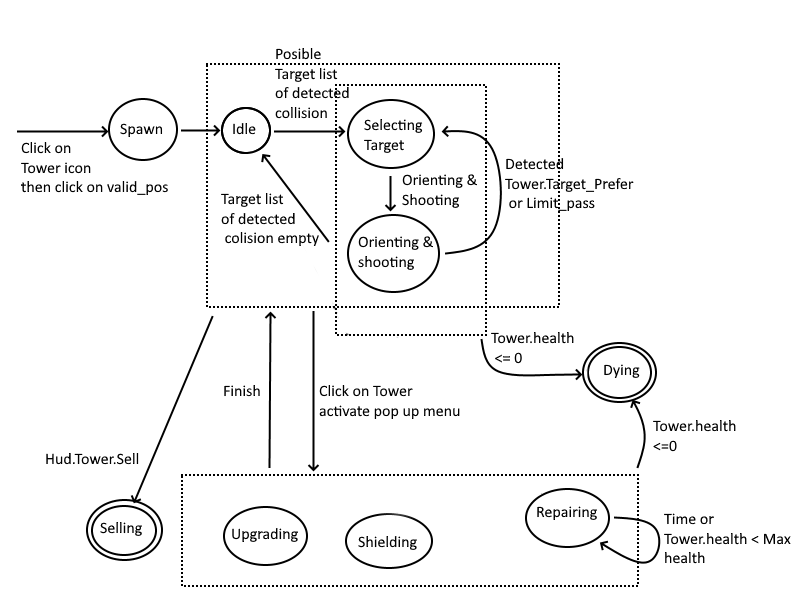
\includegraphics[width=1\textwidth]{entity-relationship/tower_movimiento.png}
    \centering
    \textcolor{Orange}{\textbf{\caption{Diagrama Entidad-Relacion Torre}}}\label{fig:1}
\end{figure}

\begin{figure}[htb]
    \centering
    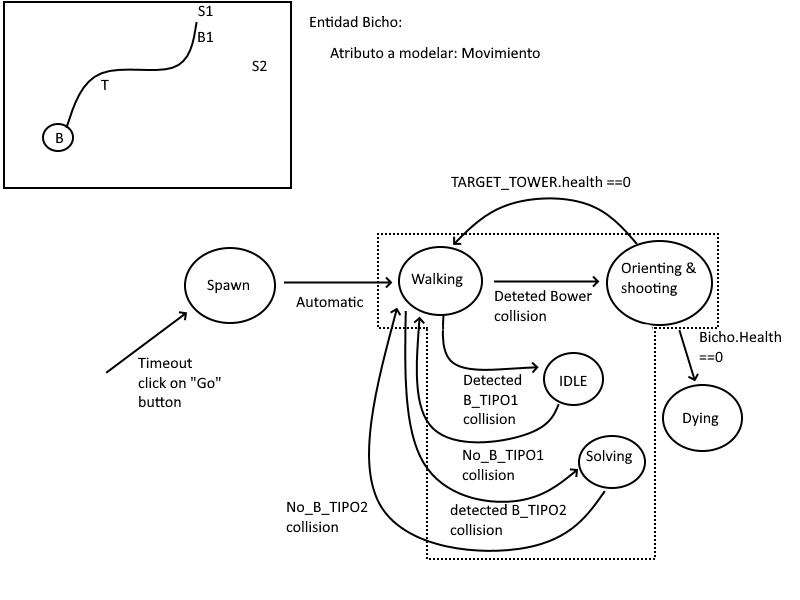
\includegraphics[width=1\textwidth]{entity-relationship/bicho_movimiento.png}
    \centering
    \textcolor{Orange}{\textbf{\caption{Diagrama Entidad-Relacion Enemigos}}}\label{fig:2}
\end{figure}

% %----------------------- Entidades y Atributos -----------------------

\cleardoublepage

%--------------------- Acciones, Interacciones y Reglas ---------------------

\section{3. Acciones, Interacciones y Reglas}

\subsection{3.1. Acciones}

\subsubsection{3.1.1. Pop-Up Actions}

\begin{itemize}
    \item \textcolor{Orange}{Vender}
    \begin{itemize}
        \item Limitaciones: vida torre mayor que 0 (no destruida)
        \item Consecuencias: espacio libre, cambio visual (torre desaparece), aumentan recursos
    \end{itemize}
    \begin{figure}[htb]
        \centering
        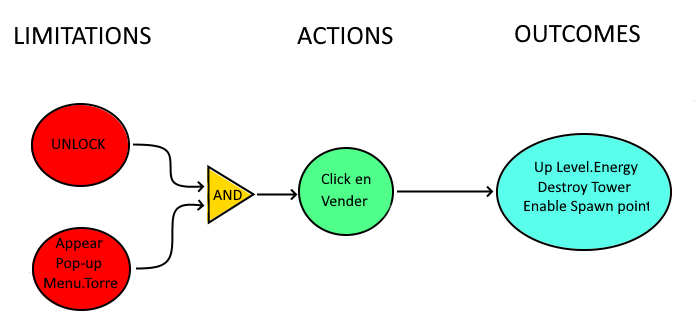
\includegraphics[width=0.7\textwidth]{action-reaction/sell.png}
        \centering
        \textcolor{Orange}{\textbf{\caption{Diagrama de la Acción Vender}}}\label{fig:3}
    \end{figure}
\end{itemize}

\begin{itemize}
    \item \textcolor{Orange}{Reparar}
    \begin{itemize}
        \item Limitaciones: vida torre mayor que 0 y menor que vida maxima, recursos suficientes
        \item Consecuencias: aumento vida torre, disminución de recursos
    \end{itemize}
    \begin{figure}[htb]
        \centering
        \includegraphics[width=0.7\textwidth]{action-reaction/reparir.png}
        \centering
        \textcolor{Orange}{\textbf{\caption{Diagrama de la Acción Reparar}}}\label{fig:4}
    \end{figure}
\end{itemize}

\begin{itemize}
    \item \textcolor{Orange}{Mejorar}
    \begin{itemize}
        \item Limitaciones: tener Torre.Nivel menor que Torre.MAX\_LEVEL, recursos suficientes, mejora desbloqueada
        \item Consecuencias: aumento de Torre.Health, disminución de recursos
    \end{itemize}
    \begin{figure}[htb]
        \centering
        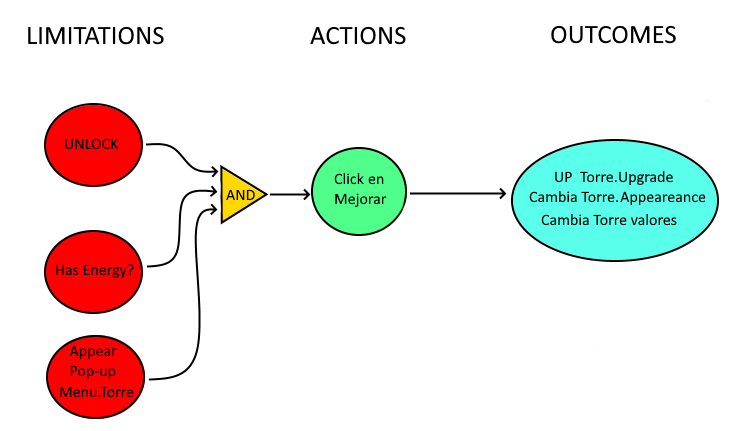
\includegraphics[width=0.7\textwidth]{action-reaction/upgrade.png}
        \centering
        \textcolor{Orange}{\textbf{\caption{Diagrama de la Acción Mejorar}}}\label{fig:5}
    \end{figure}
\end{itemize}

\begin{itemize}
    \item \textcolor{Orange}{Escudo}
    \begin{itemize}
        \item Limitaciones: recursos suficientes, habilidad desbloqueada
        \item Consecuencias: reducción de daño sobre torre, disminución de recursos
    \end{itemize}
    \begin{figure}[htb]
        \centering
        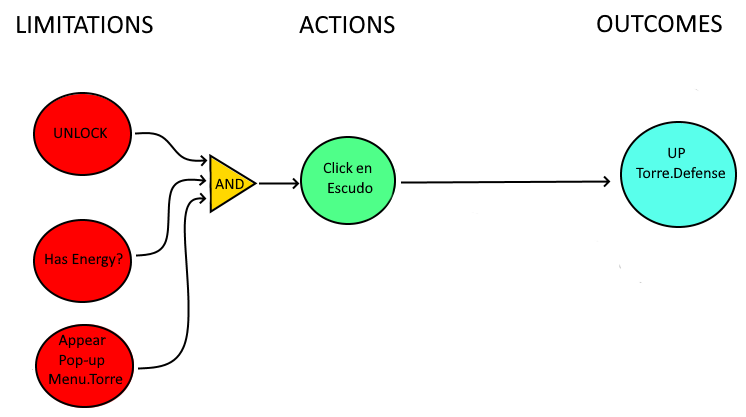
\includegraphics[width=0.7\textwidth]{action-reaction/shield.png}
        \centering
        \textcolor{Orange}{\textbf{\caption{Diagrama de la Acción Escudo}}}\label{fig:6}
    \end{figure}
\end{itemize}

\begin{itemize}
    \item \textcolor{Orange}{Controlar Base}
    \begin{itemize}
        \item Limitaciones: 
        \item Consecuencias: activa el modo de disparo de la base o Tower\_Play\_Mode
    \end{itemize}
    \begin{figure}[htb]
        \centering
        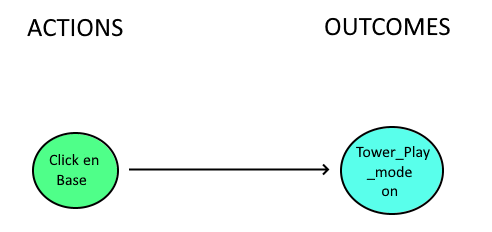
\includegraphics[width=0.7\textwidth]{action-reaction/tower_play_mode.png}
        \centering
        \textcolor{Orange}{\textbf{\caption{Diagrama de la Acción Control Baser}}}\label{fig:7}
    \end{figure}
    \begin{figure}[htb]
        \centering
        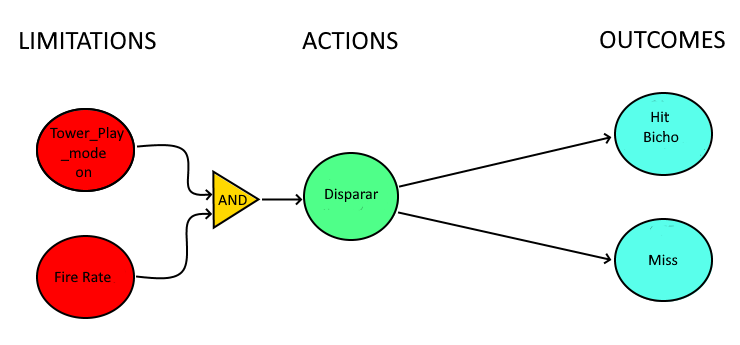
\includegraphics[width=0.7\textwidth]{action-reaction/shoot_base.png}
        \centering
        \textcolor{Orange}{\textbf{\caption{Diagrama de la Acción Dispàra}}}\label{fig:8}
    \end{figure}
\end{itemize}

\subsubsection{3.1.2. HUD Actions}

\begin{itemize}
    \item \textcolor{Orange}{Construir Torre \(O Recolector\)}
    \begin{itemize}
        \item Limitaciones: recursos suficientes, espacio libre, torre desbloqueada
        \item Consecuencias: cambio visual (nueva torre), espacio ocupado, reducción de recursos
    \end{itemize}
    \begin{figure}[htb]
        \centering
        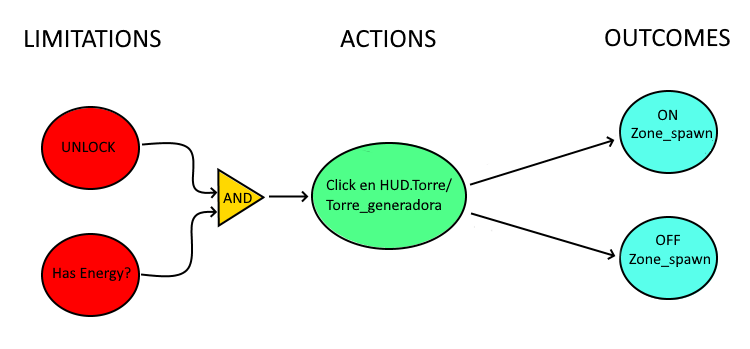
\includegraphics[width=0.7\textwidth]{action-reaction/click_hud_tower.png}
        \centering
        \textcolor{Orange}{\textbf{\caption{Diagrama de la Acción Click en Icono de Torre}}}\label{fig:9}
    \end{figure}
    \begin{figure}[htb]
        \centering
        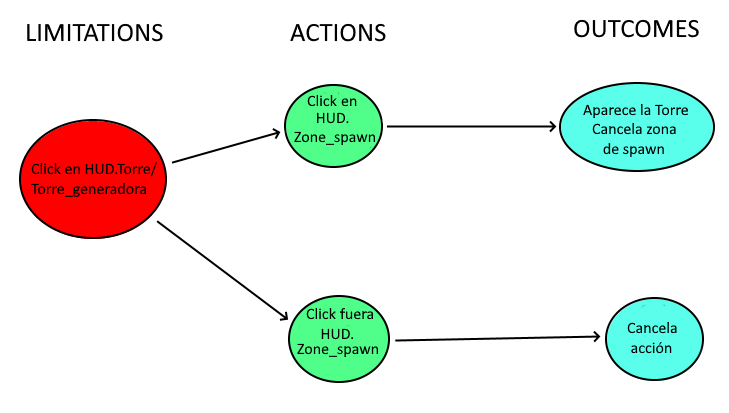
\includegraphics[width=0.7\textwidth]{action-reaction/drop_the_tower.png}
        \centering
        \textcolor{Orange}{\textbf{\caption{Diagrama de la Acción Soltar torre}}}\label{fig:10}
    \end{figure}
\end{itemize}

\begin{itemize}
    \item \textcolor{Orange}{ Seleccionar Torre)}
    \begin{itemize}
        \item Limitaciones: torre seleccionable
        \item Consecuencias: activa menú pop-up
    \end{itemize}
    \begin{figure}[htb]
        \centering
        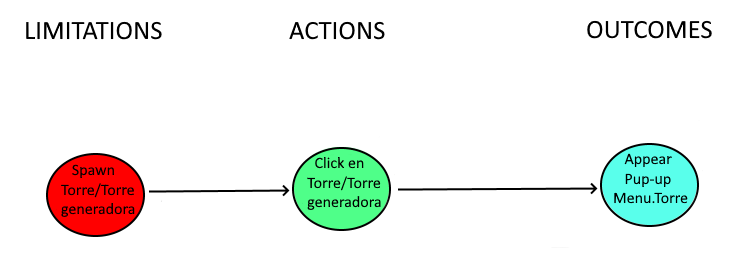
\includegraphics[width=0.7\textwidth]{action-reaction/click_on_tower.png}
        \centering
        \textcolor{Orange}{\textbf{\caption{Diagrama de la Acción Click en Torre}}}\label{fig:11}
    \end{figure}
\end{itemize}

\begin{itemize}
    \item \textcolor{Orange}{Cámara en Torre o Enemigo}
    \begin{itemize}
        \item Limitaciones: torre o enemigo seleccionable
        \item Consecuencias: cambia la posición de la camara 
    \end{itemize}
    \begin{figure}[htb]
        \centering
        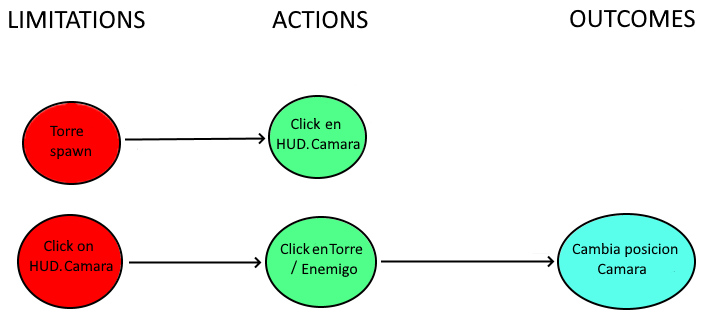
\includegraphics[width=0.7\textwidth]{action-reaction/camera.png}
        \centering
        \textcolor{Orange}{\textbf{\caption{Diagrama de la Acción Camara}}}\label{fig:12}
    \end{figure}
\end{itemize}

\begin{itemize}
    \item \textcolor{Orange}{Ataque Especial}
    \begin{itemize}
        \item Limitaciones: ataque activo \(no en tiempo de recarga\), ataque desbloqueado
        \item Consecuencias: disminución de la vida de los enemigos, activar tiempo de recarga 
    \end{itemize}
    \begin{figure}[htb]
        \centering
        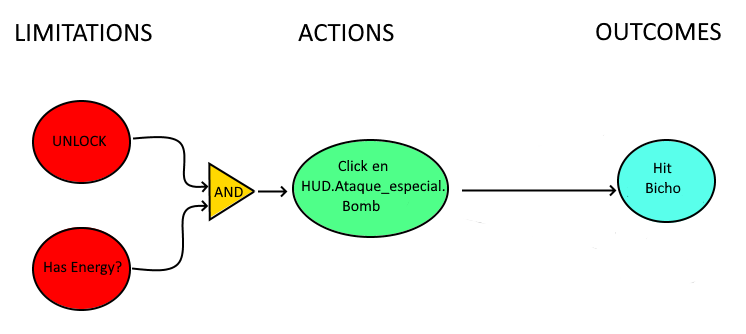
\includegraphics[width=0.7\textwidth]{action-reaction/bomb.png}
        \centering
        \textcolor{Orange}{\textbf{\caption{Diagrama de la Acción Bomba}}}\label{fig:13}
    \end{figure}
    \begin{figure}[htb]
        \centering
        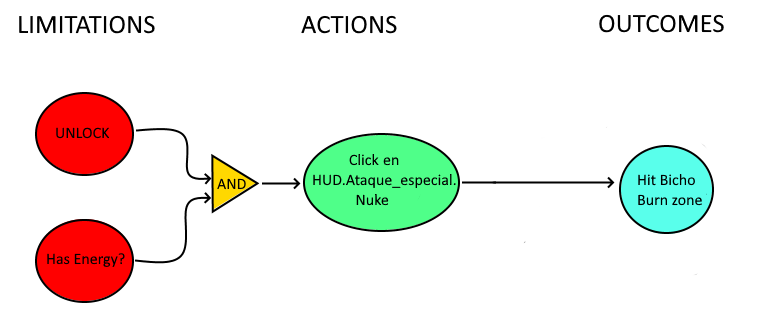
\includegraphics[width=0.7\textwidth]{action-reaction/nuke.png}
        \centering
        \textcolor{Orange}{\textbf{\caption{Diagrama de la Acción Nuke}}}\label{fig:14}
    \end{figure}
\end{itemize}

\begin{itemize}
    \item \textcolor{Orange}{Pausar el juego}
    \begin{itemize}
        \item Limitaciones:  juego activo
        \item Consecuencias: juego pausado
    \end{itemize}
\end{itemize}

\begin{itemize}
    \item \textcolor{Orange}{Reanudar Juego}
    \begin{itemize}
        \item Limitaciones:  juego pausado
        \item Consecuencias: juego reanudado
    \end{itemize}
\end{itemize}

\begin{itemize}
    \item \textcolor{Orange}{Acelerar Juego}
    \begin{itemize}
        \item Limitaciones: juego en velocidad inferior a la que se active
        \item Consecuencias: juego acelerado
    \end{itemize}
\end{itemize}

\begin{itemize}
    \item \textcolor{Orange}{Ralentizar Juego}
    \begin{itemize}
        \item Limitaciones:  juego en velocidad superior a la que se active
        \item Consecuencias: se ralentiza el juego
    \end{itemize}
\end{itemize}

\subsubsection{3.1.3. Research Actions}

\begin{itemize}
    \item \textcolor{Orange}{Elegir Mejora}
    \begin{itemize}
        \item Limitaciones: tener XP, tener el nivel previo de la mejora si lo hay
        \item Consecuencias: se selecciona la mejora, sin hacerse efectiva 
    \end{itemize}
\end{itemize}

\begin{itemize}
    \item \textcolor{Orange}{Confirmar Mejora}
    \begin{itemize}
        \item Limitaciones: haber seleccionado la mejora, pulsar el botón de aceptación
        \item Consecuencias: se agrega la mejora, se vuelve a la pantalla de mapa
    \end{itemize}
\end{itemize}

\begin{itemize}
    \item \textcolor{Orange}{Cancelar Mejora}
    \begin{itemize}
        \item Limitaciones: pulsar el botón de cancelación
        \item Consecuencias: se vuelve a la pantalla de mapa, no se confirman las mejoras elegidas
    \end{itemize}
\end{itemize}

\subsubsection{3.1.4. Map Actions}

\subsubsection{3.1.5. Difficulty Actions}

\subsection{3.2. Interacciones}

\subsection{3.3. Reglas}

% %--------------------- Acciones, Interacciones y Reglas ---------------------

\end{document}

% %----------------------- Document -----------------------